\documentclass{article}
\usepackage[utf8]{inputenc}
\usepackage{amsmath,blkarray}
\usepackage{tikz}
\usetikzlibrary{shapes,arrows,positioning}
\title{Assignment 3}
\author{AI22MTECH02003 - Shrey Satapara}

\tikzset{
    place/.style={
        circle,
        thick,
        draw=black,
        fill=gray!50,
        minimum size=6mm,
    },
        state/.style={
        circle,
        thick,
        draw=blue!75,
        fill=blue!20,
        minimum size=6mm,
    },
}

\begin{document}

\maketitle

\paragraph{Q 51 (June 2018)}
Consider a Markov Chain having state space \(S = {1,2,3,4}\) with a transation probablity matrix \(P = (p_{i,j})\) given by 


\[
\mathbf{P} = 
        \begin{blockarray}{ccccc}
         & 1   & 2   & 3 & 4 \\
        \begin{block}{r||rrrr||}
        1 & \frac{1}{2} & 0 & \frac{1}{2} & 0\\
        2 & \frac{1}{4} & \frac{1}{4} & \frac{1}{4} & \frac{1}{4}\\
        3 & \frac{1}{3}   & 0   & \frac{1}{3}   & \frac{1}{3}\\
        4 & \frac{1}{2}   & 0   & \frac{1}{2}   & 0\\
        \end{block}
    \end{blockarray}
\] Then \\\\
1.\quad \( \lim_{n\to\infty} p_{2,2}^{(n)} = 0, \quad\quad \sum_{n=0}^{\infty} p_{2,2}^{(n)} = \infty \)
\\
2.\quad \( \lim_{n\to\infty} p_{2,2}^{(n)} = 0, \quad\quad \sum_{n=0}^{\infty} p_{2,2}^{(n)} < \infty \)
\\
3.\quad \( \lim_{n\to\infty} p_{2,2}^{(n)} = 1, \quad\quad \sum_{n=0}^{\infty} p_{2,2}^{(n)} = \infty \)
\\
4.\quad \( \lim_{n\to\infty} p_{2,2}^{(n)} = 1, \quad\quad \sum_{n=0}^{\infty} p_{2,2}^{(n)} < \infty \)

\paragraph{Solution}
A markov chain having state space \(S = {1,2,3,4}\) and transation probablity matrix \(P = (p_{i,j})\) is 
\[
\mathbf{P} = 
        \begin{blockarray}{ccccc}
         & 1   & 2   & 3 & 4 \\
        \begin{block}{r||rrrr||}
        1 & \frac{1}{2} & 0 & \frac{1}{2} & 0\\
        2 & \frac{1}{4} & \frac{1}{4} & \frac{1}{4} & \frac{1}{4}\\
        3 & \frac{1}{3}   & 0   & \frac{1}{3}   & \frac{1}{3}\\
        4 & \frac{1}{2}   & 0   & \frac{1}{2}   & 0\\
        \end{block}
    \end{blockarray}
\]

\paragraph{Limiting Probabilities:} \( \lim_{n\to\infty} p_{i,j}^{(n)} \) is a probablity of coming to j from i in n steps, where \(n\to\infty\). 
\\\\
Let's look at state transition diagram \newpage
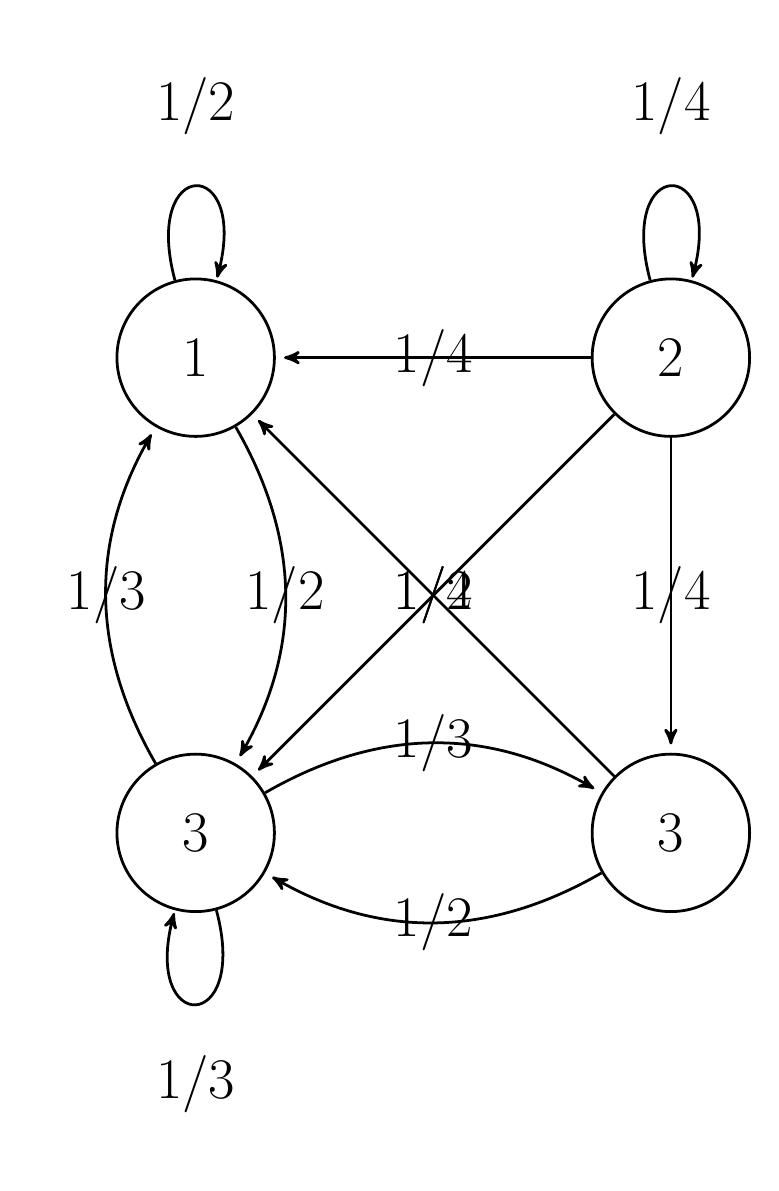
\begin{tikzpicture}[->,>=stealth',shorten >=3pt, line width=1pt, 
                                  node distance=4cm, style ={minimum size=20mm}]
\tikzstyle{every node}=[font=\huge]


\node [circle, draw] (a) {1};
\node [circle, draw] (b) [right=of a] {2};
\node [circle, draw] (c) [below=of a] {3};
\node [circle, draw] (d) [below=of b] {3};
\path  (a) edge [loop above] node {1/2} (a);
\path  (b) edge [loop above] node {1/4} (b);
\path  (c) edge [loop below] node {1/3} (c);

\path[->] (a) edge [bend left] node {1/2} (c);

\path[->] (b) edge node {1/4} (a);
\path[->] (b) edge node {1/4} (c);
\path[->] (b) edge node {1/4} (d);

\path[->] (c) edge [bend left] node {1/3} (a);
\path[->] (c) edge [bend left] node {1/3} (d);

\path[->] (d) edge node {1/2} (a);
\path[->] (d) edge [bend left] node {1/2} (c);
\end{tikzpicture}

\\ 
By looking at state 2 in above diagram we can say that it is a transient state. and
\begin{gather*}
    p_{2,2}^{(1)} = \frac{1}{4} \\
    p_{2,2}^{(2)} = \frac{1}{4}*\frac{1}{4} = \left( \frac{1}{4} \right)^2 \\
    p_{2,2}^{(3)} = \left( \frac{1}{4} \right)^3
\end{gather*}
and so on. For \(n\to\infty\)
\begin{equation}
\begin{split}
    p_{2,2}^{(n)} & = \left( \frac{1}{4} \right)^n \\
    & = \left( \frac{1}{4} \right)^\infty \\
    & = 0
\end{split}    
\end{equation}
\textbf{Hence, } \(\lim_{n\to\infty} p_{2,2}^{(n)} = 0\)
\\\\
Now for second part \quad \(\sum_{n=0}^{\infty} p_{2,2}^{(n)}\)

\begin{equation}
    \begin{split}
    \sum_{n=0}^{\infty} p_{2,2}^{(n)} \quad & = \quad p_{2,2}^{(1)} \quad +  \quad p_{2,2}^{(2)} \quad  + \quad p_{2,2}^{(3)} \quad + \quad \dots \\
    & = \quad \left( \frac{1}{4} \right) \quad + \quad \left( \frac{1}{4} \right)^2 \quad + \quad \left( \frac{1}{4} \right)^3 \quad + \quad \dots \\
    & = \frac{\frac{1}{4}}{1 - \frac{1}{4}} \\
    & = \frac{\frac{1}{4}}{\frac{3}{4}} \\
    & = \frac{1}{3} \\
    & < \infty
    \end{split}
\end{equation}
Means, \quad \(\sum_{n=0}^{\infty} p_{2,2}^{(n)} = \frac{1}{3} < \infty\)

Here we have \quad \(\lim_{n\to\infty} p_{2,2}^{(n)} = 0\) and \quad \(\sum_{n=0}^{\infty} p_{2,2}^{(n)} = \frac{1}{3} < \infty\) \\\\
\textbf{Hence, Option 2 is the correct answer}

\end{document}